\documentclass[prb,9pt,notitlepage]{revtex4-1}
%\documentclass[a4paper,twocolumn,9pt]{article}

%\usepackage{geometry}
%\geometry{a4paper,top=2.5cm,bottom=2cm,inner=1.5cm,outer=1.5cm}

\usepackage{mwe}% just for the example content
\usepackage{color}
\usepackage{latexsym,amsmath}
\usepackage{physics}
\usepackage{listings}
\usepackage[dvipsnames]{xcolor}
\usepackage{parskip}
\usepackage{hyperref}
\usepackage{amsmath}
\usepackage{bbm}
%\usepackage{dblfloatfix}
%\usepackage{subfig}
\definecolor{linkcolor}{rgb}{0,0,0.65}%hyperlink
\definecolor{shadecolor}{rgb}{0.93, 0.93, 0.93}
%\usepackage[pdftex,colorlinks=true, pdfstartview=FitV, linkcolor= linkcolor, citecolor= linkcolor, urlcolor= linkcolor, hyperindex=true,hyperfigures=true]{hyperref} %hyperlink%
%\usepackage[backend=biber, sorting=ynt]{biblatex}
%\usepackage{ragged2e} % to justify caption
%\addbibresource{bibliography.bib}
 \usepackage{booktabs}

\usepackage[T1]{fontenc}
\usepackage{xcolor}
\usepackage{lmodern}
\usepackage{listings}
\lstset{language=[95]Fortran,
  backgroundcolor=\color{shadecolor},
  basicstyle=\ttfamily,
  keywordstyle=\color{blue},
  commentstyle=\color{gray},
  stringstyle=\color{red},
  showstringspaces=false
  %morecomment=[l]{!\ }% Comment only with space after !
}

\usepackage{tabularx}

\usepackage{fancyhdr}
\pagestyle{fancyplain}% <- use fancyplain instead fancy
\fancyhf{}
\fancyhead[R]{\today}
\fancyhead[L]{Alessandro Lambertini}
\fancyfoot[L]{Quantum information and computing}
\fancyfoot[C]{Report 2}
\fancyfoot[R]{\thepage}

\renewcommand{\headrulewidth}{0pt}

\usepackage{float}
\usepackage{siunitx}




\begin{document}
\title{Quantum information and computing: Exercises report, week 4. \\ Multi-run script \& Automated fits }

\author{Alessandro Lambertini}


\date{\today}

\begin{abstract}
Through the exercise of this week,  we study from a numerical perspective the 1-D quantum Ising model in a transverse field. In particular, we have to implement a program that is able to effectively write the hamiltonian of the system in its matrix form and diagonalize it for different values of $N$, the number of spins that form the system, and for different values of $\lambda$, the interaction strenght.
\end{abstract}

\maketitle

\section{Theory}
The Hamiltonian that describes properly our system is:
\begin{equation}
  H = \sum_{i=1}^N \sigma_z^{(i)} + \lambda\sum_{i=1}^{N-1}\sigma_x^{i+1}\sigma_x^{i}
\end{equation}
where $\sigma_z$ and $\sigma_x$ are Pauli's matrices and the two terms under the summation signs are expanded as follows:
\begin{eqnarray}
\nonumber\\
\sigma_z \otimes \mathbbm{1}_2\otimes\dots\otimes\mathbbm{1}_N + \mathbbm{1}_1\otimes\sigma_z\otimes \mathbbm{1}_3\otimes\dots\otimes\mathbbm{1}_N+\dots+\mathbbm{1}_1\otimes\mathbbm{1}_2\otimes\dots\otimes\sigma_z \label{first_term}\\\nonumber
\\
\sigma_x \otimes \sigma_x\mathbbm{1}_3\otimes\dots\otimes\mathbbm{1}_N + \mathbbm{1}_1\otimes\sigma_x\otimes\sigma_x \mathbbm{1}_4\otimes\dots\otimes\mathbbm{1}_N+\dots+\mathbbm{1}_1\otimes\mathbbm{1}_2\otimes\dots\otimes\sigma_x\otimes\sigma_x \label{second_term} \\\nonumber
\end{eqnarray}
We will compare, qualitatively, our solutions with the one analitically obtained under the mean field assumptions, that is:
\begin{equation}
\begin{cases}
E_0 = -1-\frac{\lambda^2}{4} & \lambda \in [-2:2] \\
E_0 = -\abs{\lambda} & \lambda \notin [-2:2]
\end{cases}
\end{equation}

\section{Code development}
In order to accomplish the tasks I wrote and exploited some subroutines that are located in the \textit{ex09\_module} written in the file \textit{ex09\_module.f90}. First of all, I implemented a subroutine that performs the tensor product between two matrices \textit{mat\_1} and \textit{mat\_2}, as follows:
\begin{lstlisting}
!!!!!!!!!!!!!!!!! tensor product of two complex matrices !!!!!!!!!!!!!!!!!
subroutine tensor_product(mat_1, mat_2, mat_prod)
    complex(kind=8), dimension(:,:):: mat_1, mat_2
    complex(kind=8), dimension(:, :), allocatable :: mat_prod
    integer :: ii, jj
    integer, dimension(2) :: dimm_1, dimm_2

    dimm_1 = shape(mat_1)
    dimm_2 = shape(mat_2)

    allocate (mat_prod(dimm_1(1)*dimm_2(1), dimm_1(1)*dimm_2(1)))
    do ii=1, dimm_1(1)
        do jj=1, dimm_1(1)
            mat_prod((ii-1)*dimm_2(1)+1:ii*dimm_2(1), (jj-1)*dimm_2(1)+1:jj*&
            dimm_2(1))=mat_1(ii,jj)*mat_2
        end do
    end do
  end subroutine tensor_product
!!!!!!!!!!!!!!!!!!!!!!!!!!!!!!!!!!!!!!!!!!!!!!!!!!!!!!!!!!!!!!!!!!!!!!!!
\end{lstlisting}
With this tool, I proceeded implementing the two very similar subroutines that compute each term under the summation signs (\ref{first_term}) (\ref{second_term}). These subroutines take as arguments the number of spins that make un the system and the indexes of the position of the spin under exam. I tested the two subroutines with the results obtained for $N=2$ and $N=3$ computed by hand. Here below I report the full code of the first of these two subroutines, the one that computes $\sigma_z^{(i)}$.
\begin{lstlisting}
!!!!!!!!!!!!!!!!!!! compute sigma_z^(i) !!!!!!!!!!!!!!!!!!!
subroutine sigma_z_i(N,ii,mat_prod)
  complex(kind=8), dimension(:,:), allocatable :: prod_id, prod_1,&
  prov_prod, mat_prod
  complex(kind=8), dimension(2,2) :: sigma_z, identity
  integer :: N, ii,jj

  allocate(prod_id(2,2))

  sigma_z(1,1) = (1,0)
  sigma_z(1,2) = (0,0)
  sigma_z(2,1) = (0,0)
  sigma_z(2,2) = (-1,0)

  identity(1,1) = (1,0)
  identity(1,2) = (0,0)
  identity(2,1) = (0,0)
  identity(2,2) = (1,0)

  prod_id(1,1) = (1,0)
  prod_id(1,2) = (0,0)
  prod_id(2,1) = (0,0)
  prod_id(2,2) = (1,0)

  do jj = 1, ii-2
    call tensor_product(prod_id, identity, prov_prod)
    deallocate(prod_id)
    prod_id = prov_prod
    deallocate(prov_prod)
  end do

  if ( ii .eq. 1) then
    call tensor_product(sigma_z,prod_id,prov_prod)
    deallocate(prod_id)
    prod_id = prov_prod
    deallocate(prov_prod)
  else
    call tensor_product(prod_id,sigma_z,prov_prod)
    deallocate(prod_id)
    prod_id = prov_prod
    deallocate(prov_prod)
  end if

  if ( ii .eq. 1) then
    do jj = 1, N-2
      call tensor_product(prod_id, identity, prov_prod)
      deallocate(prod_id)
      prod_id = prov_prod
      deallocate(prov_prod)
    end do
  else
    do jj = 1, N-ii
      call tensor_product(prod_id, identity, prov_prod)
      deallocate(prod_id)
      prod_id = prov_prod
      deallocate(prov_prod)
    end do
  end if

  mat_prod = prod_id
  deallocate(prod_id)

end subroutine sigma_z_i
!!!!!!!!!!!!!!!!!!!!!!!!!!!!!!!!!!!!!!!!!!!!!!!!!!!!!!!!!!!!!!!!!!!!!!!!
\end{lstlisting}
At this point, I have been able to make use of these subroutines to write a compact one that, given the number of spins and the interaction strenght outputs the matrix form of the Hamiltonian described above. Essentially, in this subroutine the sums are performed.
\begin{lstlisting}
!!!!!!!!!!!!!!!!!!! compute the hamiltonian of the Ising !!!!!!!!!!!!!!!!!!!
    !!!!!!!!!!!!!!!!!!!!!! model for N particles in t f !!!!!!!!!!!!!!!!!!!!!!
    subroutine H_ising_np_tr(N,lambda,ham)
      complex(kind=8), dimension(:,:), allocatable :: mat_prod,int_term,ham,&
      mat_prod_1,mat_prod_2,tr_term
      real(kind=8) :: lambda
      integer :: N, ii,jj

      allocate(int_term(2**N,2**N),ham(2**N,2**N),tr_term(2**N,2**N))
      int_term = (0,0)
      tr_term = (0,0)
      do ii=1,N
        call sigma_z_i(N,ii,mat_prod)
        int_term = int_term + mat_prod
        deallocate(mat_prod)
      end do

      do ii=1,N-1
        call sigma_xx_i(N,ii,mat_prod)
        tr_term = tr_term + mat_prod
        deallocate(mat_prod)
      end do
      ham = lambda*int_term + tr_term
    end subroutine H_ising_np_tr

    !!!!!!!!!!!!!!!!!!!!!!!!!!!!!!!!!!!!!!!!!!!!!!!!!!!!!!!!!!!!!!!!!!!!!!!!
\end{lstlisting}
With these tools I was able to exploit the previously written subroutine to diagonalize an hermitian matrix and solve the problem.




\section{Results}
Here below is shown the program implemented to obtain some results out of the tools presented above. This program, after having choose the  maximum number of spins $N$ for which make the computation, and the range and number of values in which $\lambda$ can span, produces $N$ files in output. The first one, named \textit{gs\_N.txt}, represents the first eigenvalues for each number of spins from $2$ to $N$, as a function of $\lambda$. The other $N-1$ files, named \textit{"firstfoureigv\_(N).txt}, where $(N)$ takes all the different values from 2 to N, describe the first four eigenvalues as a function of $\lambda$.
\begin{lstlisting}
program ex09
  use ex09module
  implicit none

complex(kind=8), dimension(:,:), allocatable :: sigma_z, sigma_x, ham
real(kind=8), dimension(:), allocatable :: eigv,lambda_i
real(kind=8), dimension(:,:), allocatable :: ground_states,four_eigv
real(kind=8) :: start,end,step,lambda_max
integer :: N, ii,jj,M,N_max
character(len=1024) :: filename

M = 100
N_max = 10
lambda_max = 3
allocate(lambda_i(M),ground_states(M,N_max))

step = lambda_max/real(M-1,8)

do ii=1,M
  lambda_i(ii) = 0+(ii-1)*step
end do

do N=2,N_max
  call cpu_time(start)
  allocate(four_eigv(M,4))
  do ii=1,M
    call H_ising_np_tr(N,lambda_i(ii),ham)
    call diag_hermit_matrix(ham,eigv)
    ground_states(ii,N-1) = eigv(1)/(N-1)
    four_eigv(ii,1) = eigv(1)/(N-1)
    four_eigv(ii,2) = eigv(2)/(N-1)
    four_eigv(ii,3) = eigv(3)/(N-1)
    four_eigv(ii,4) = eigv(4)/(N-1)
    deallocate(ham,eigv)
    write(*,*) 'N=',N,', M=',ii
  end do
  if ( N .lt. 10 ) then
    write (filename, "(A14,I1,A4)") "firstfoureigv_", N,'.txt'
  else
    write (filename, "(A14,I2,A4)") "firstfoureigv_", N,'.txt'
  end if
  call vec_and_col_on_file(filename,four_eigv,4,lambda_i)
  deallocate(four_eigv)
  call cpu_time(end)
  write(*,*) 'N=',N,' done, time needed:',end-start
end do

call vec_and_col_on_file('gs_N.txt',ground_states,N_max-1,lambda_i)
end program ex09
\end{lstlisting}
The maximum $N$ that my pc was able to reach is 12, but to accomplish the task it took more than three hours, more precisely $11730$ s.

The results obtained are then exploited to produce some plots with gnuplot. In fig.\ref{ground_states} we see the values of the first eigenvalue with $N$ varying from 2 to 12, together with the exact solution of the problem under the mean field assumptions. As N increases our solution seems to collapse to the m.f. one. This is reasonable because with the mean field solution we approximate the system in the thermodynamic limit. In fig.\ref{fig:foobar} we can see the behaviour of the first four energy levels of the system for 4 different N. We can see that switching on the interaction ($\lambda\ne 0$) cause the degeneracy to vanish. We observe also a trend, for the energy levels other than the ground state, for which increasing N they tend to be more close to each other.

\begin{figure}[h]
    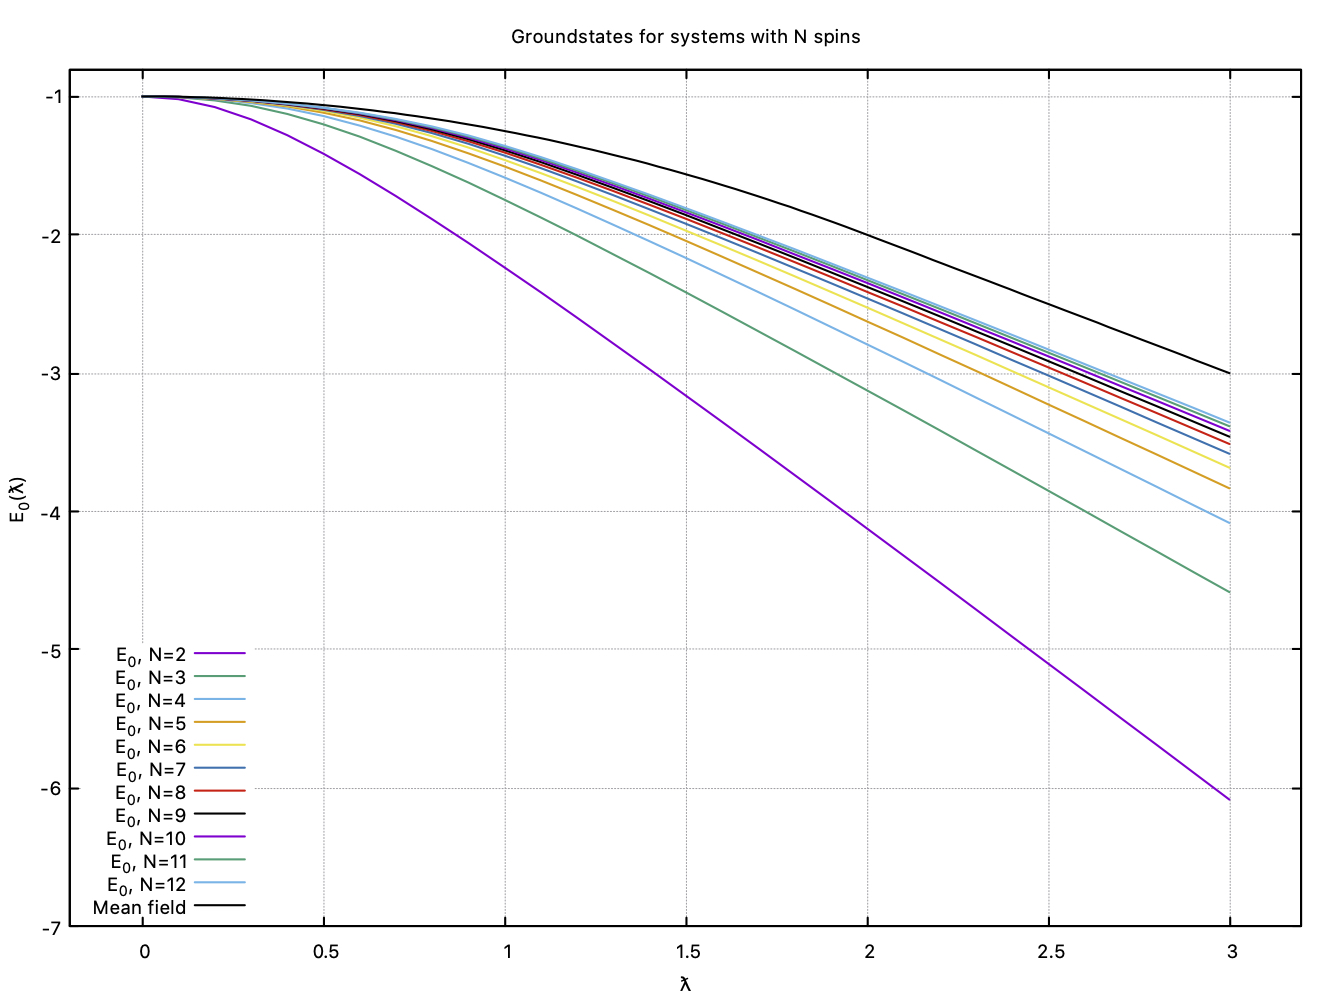
\includegraphics[width=.50\textwidth]{ground_states}\hfill
%    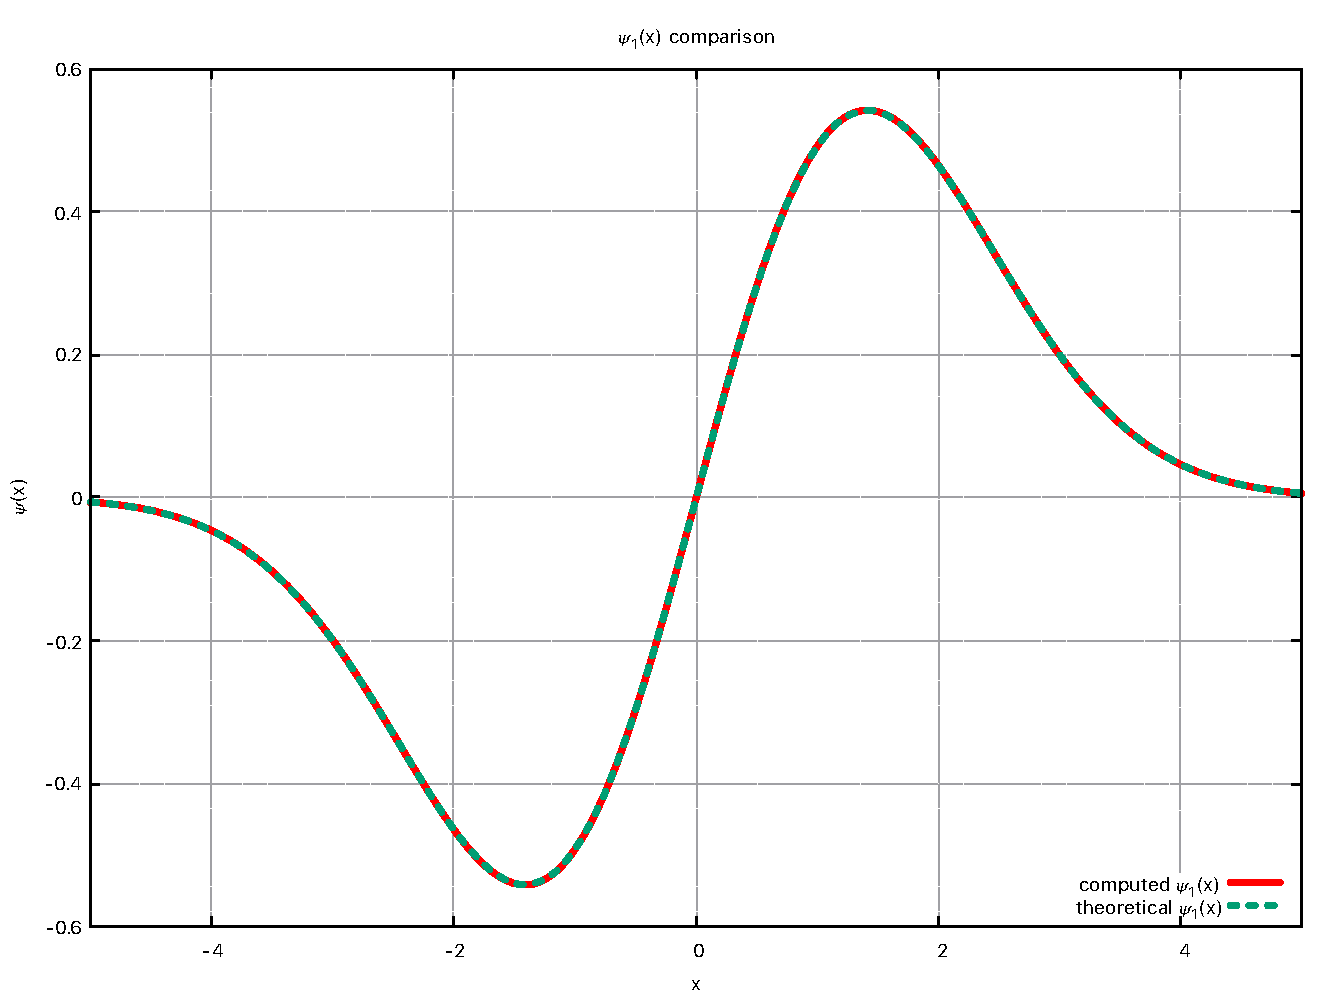
\includegraphics[width=.45\textwidth]{psi_1}\hfill
%    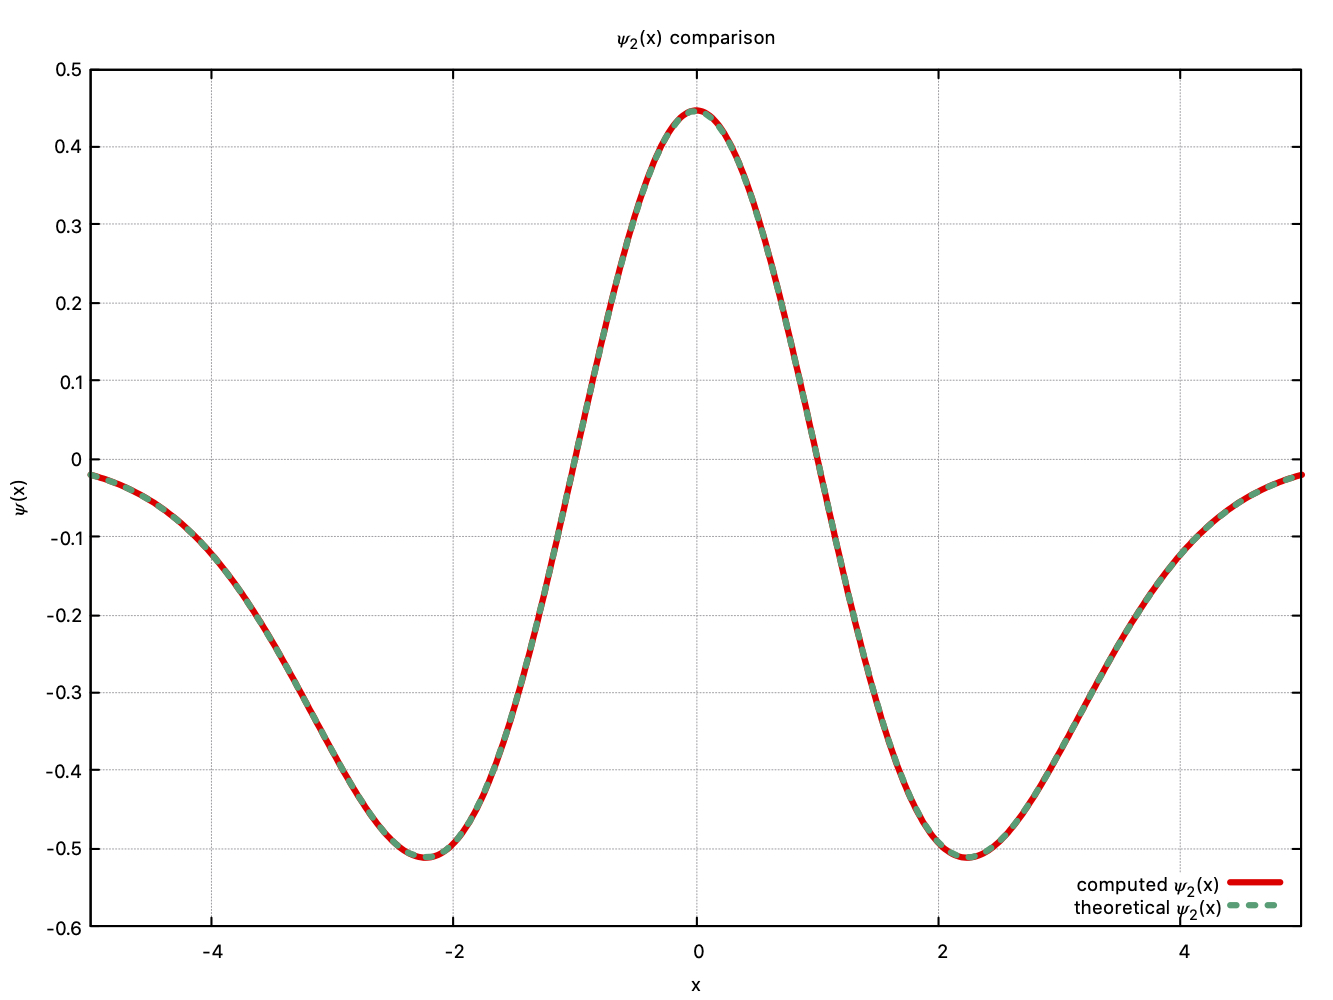
\includegraphics[width=.45\textwidth]{psi_2}
%%    \\[\smallskipamount]
%%    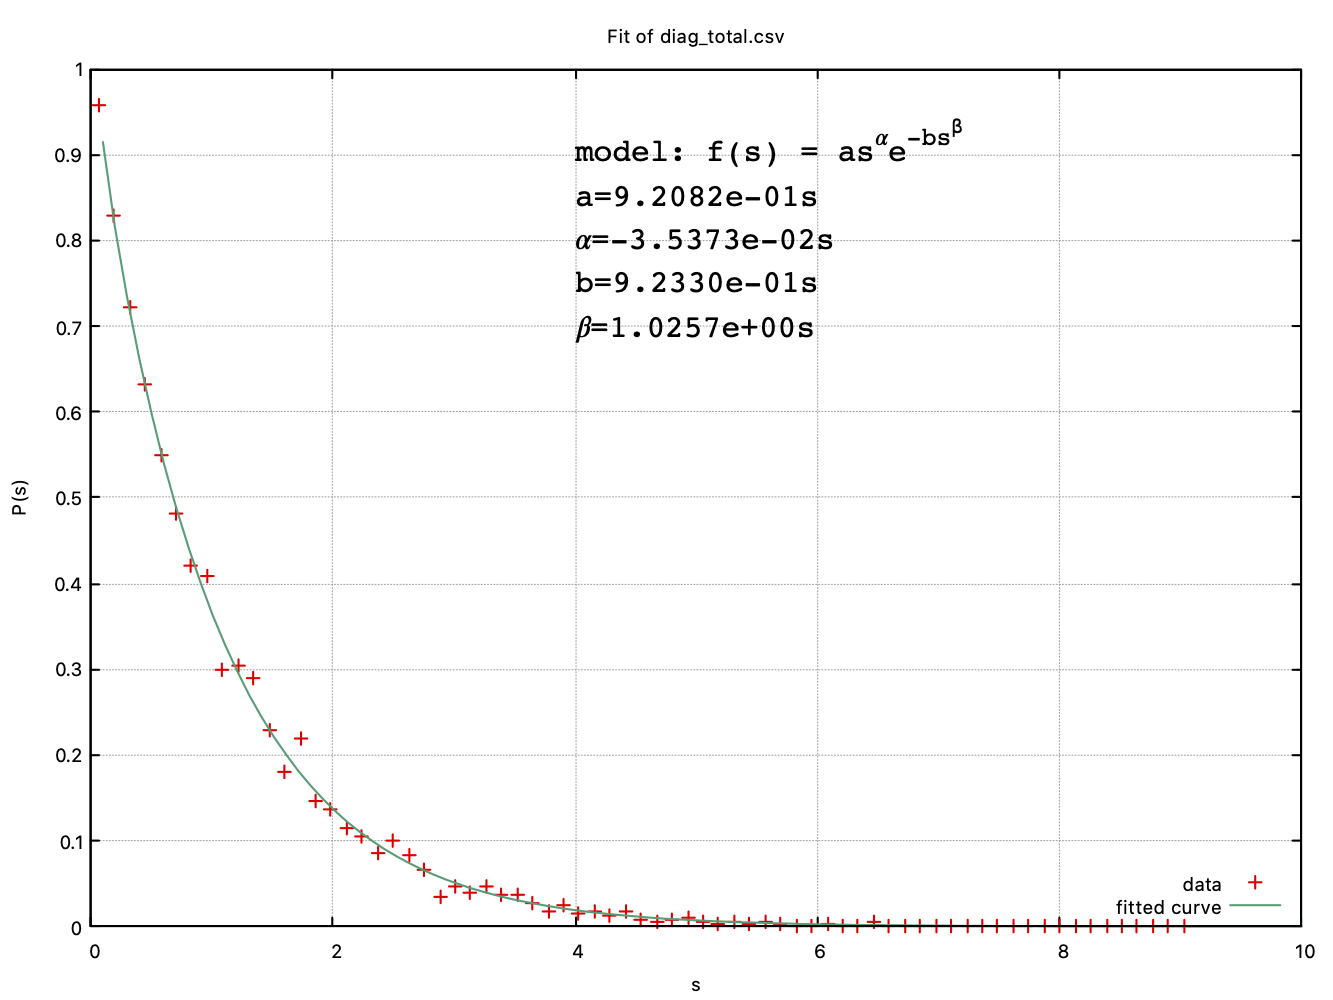
\includegraphics[width=.33\textwidth]{diag_total}\hfill
%%    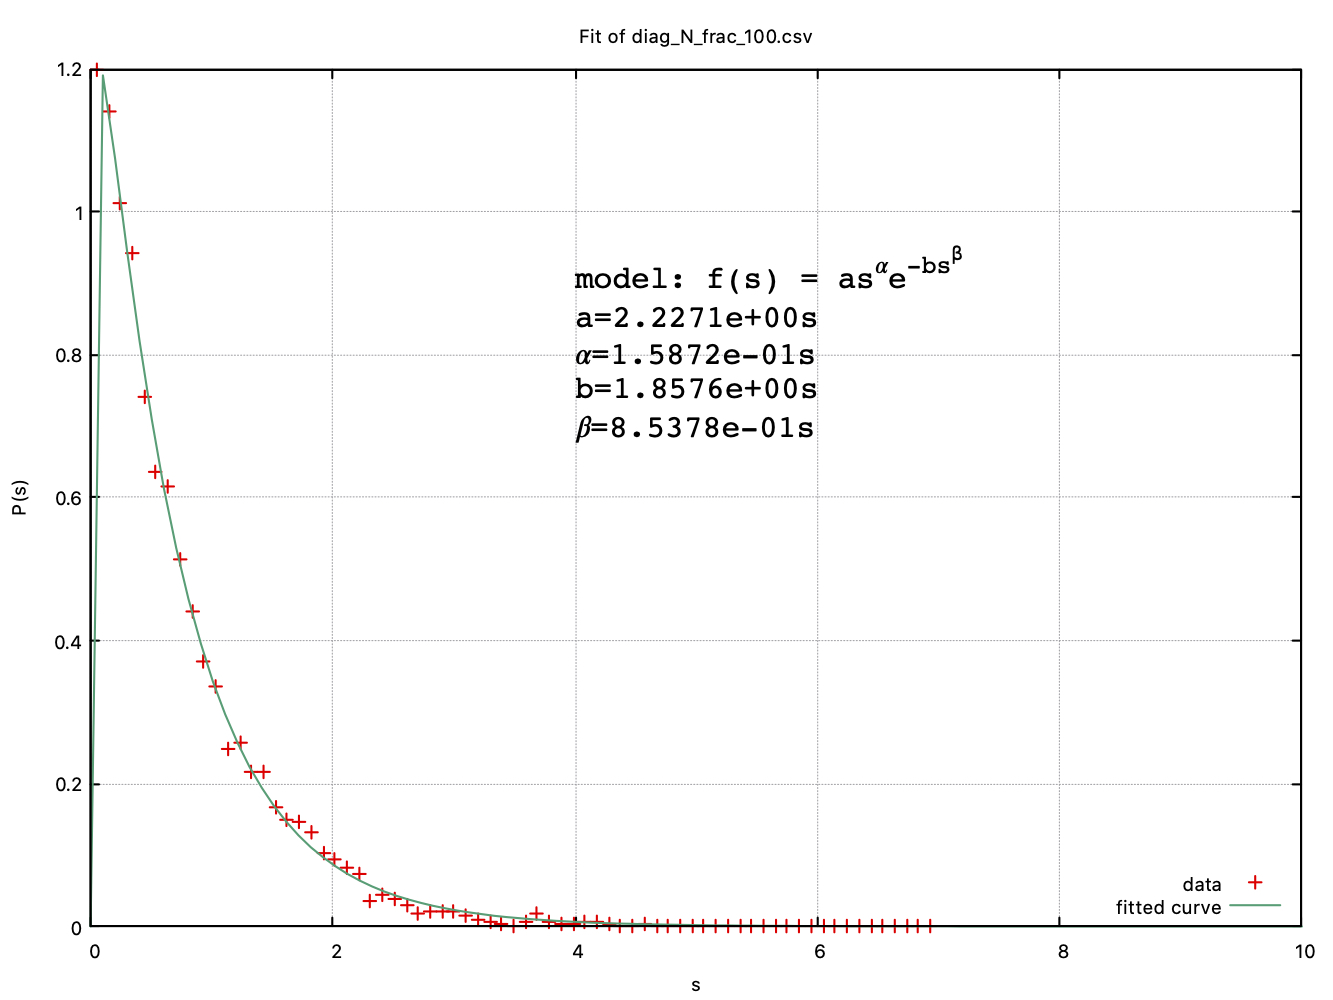
\includegraphics[width=.33\textwidth]{diag_N_frac_100}\hfill
%%    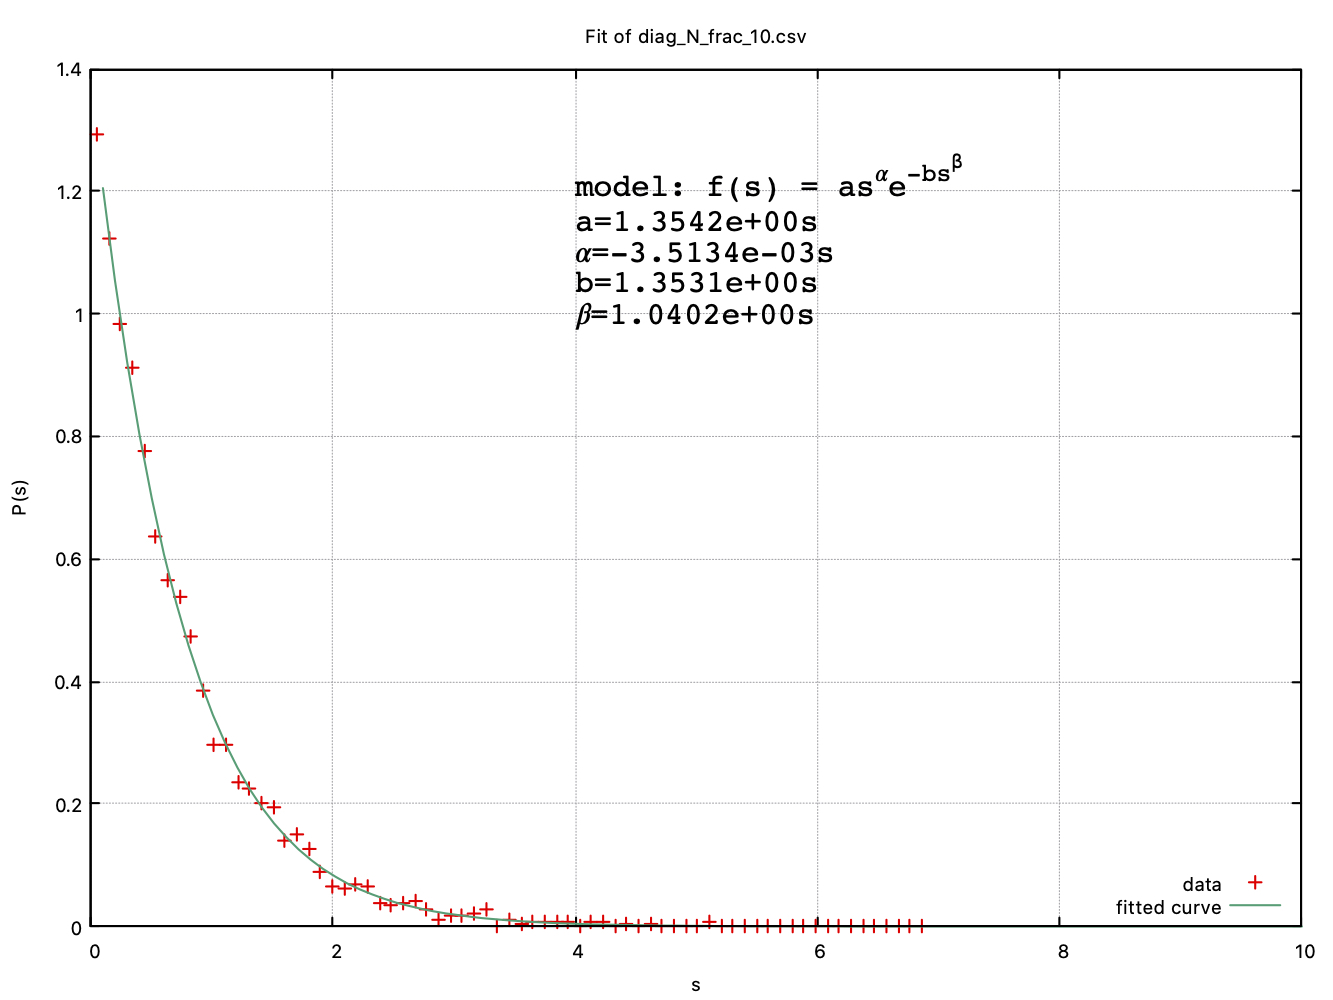
\includegraphics[width=.33\textwidth]{diag_N_frac_10}
    \caption{The ground state of the system for different values of $N$ as a function of $\lambda$}\label{ground_states}
\end{figure}

\begin{figure}[H]
    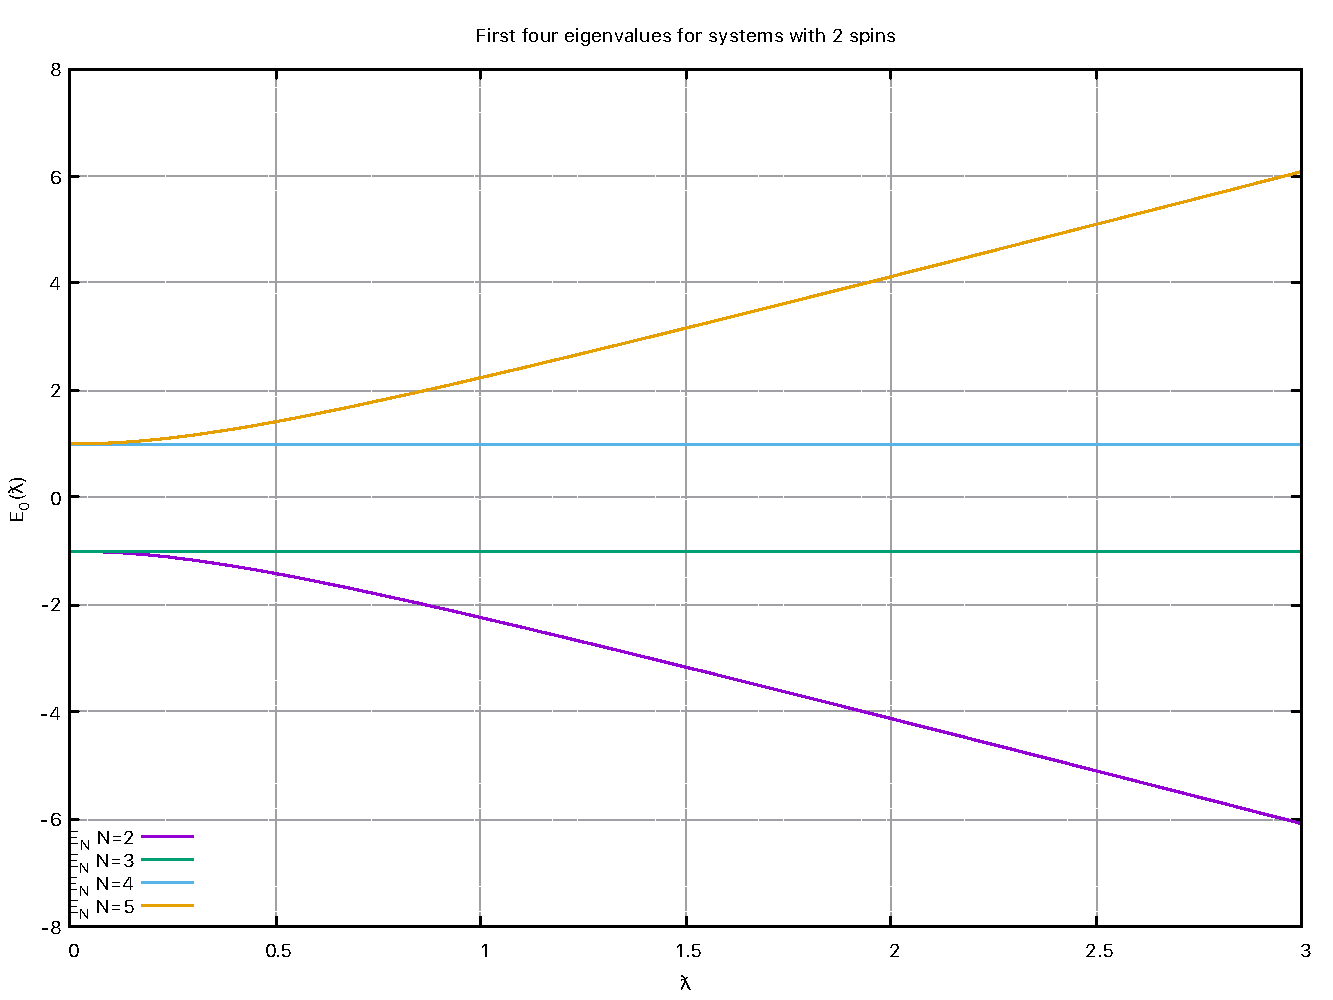
\includegraphics[width=.40\textwidth]{firstfour_2}\hfill
    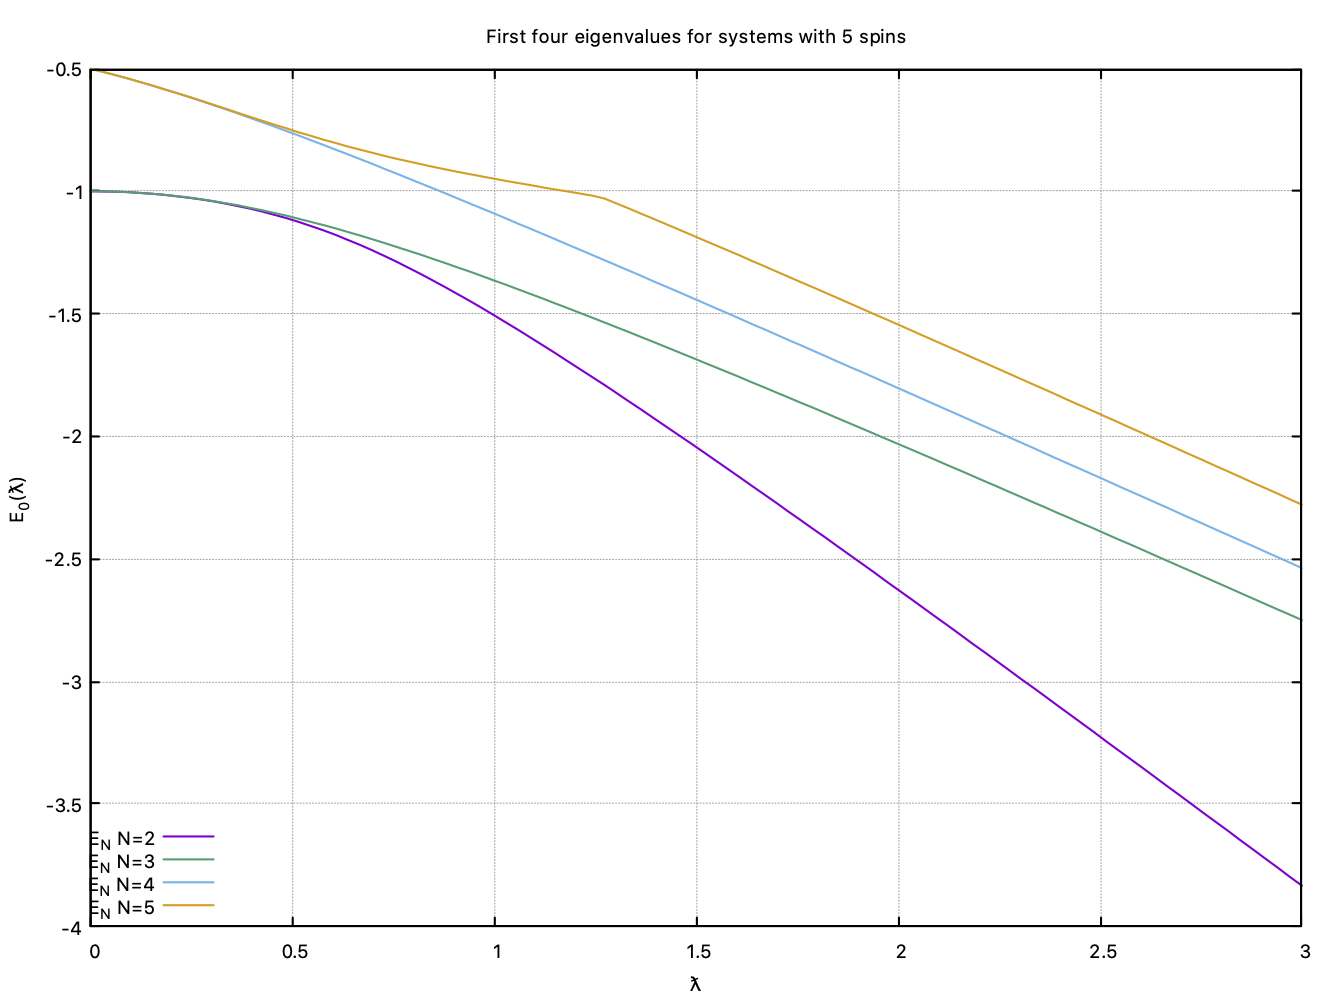
\includegraphics[width=.40\textwidth]{firstfour_5}\hfill
%    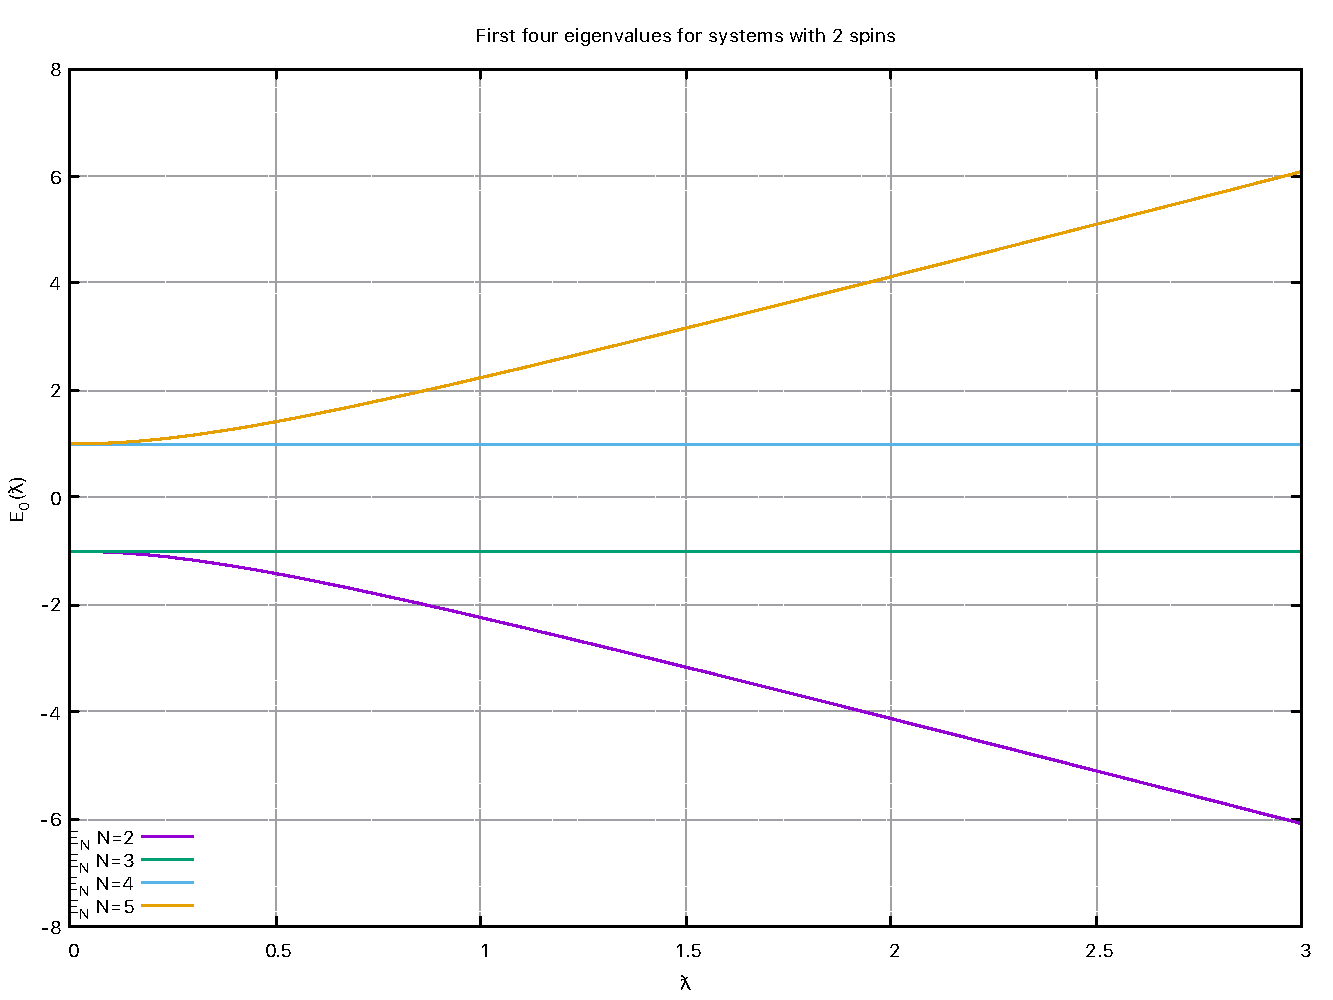
\includegraphics[width=.45\textwidth]{firstfour_2}
    \\[\smallskipamount]
    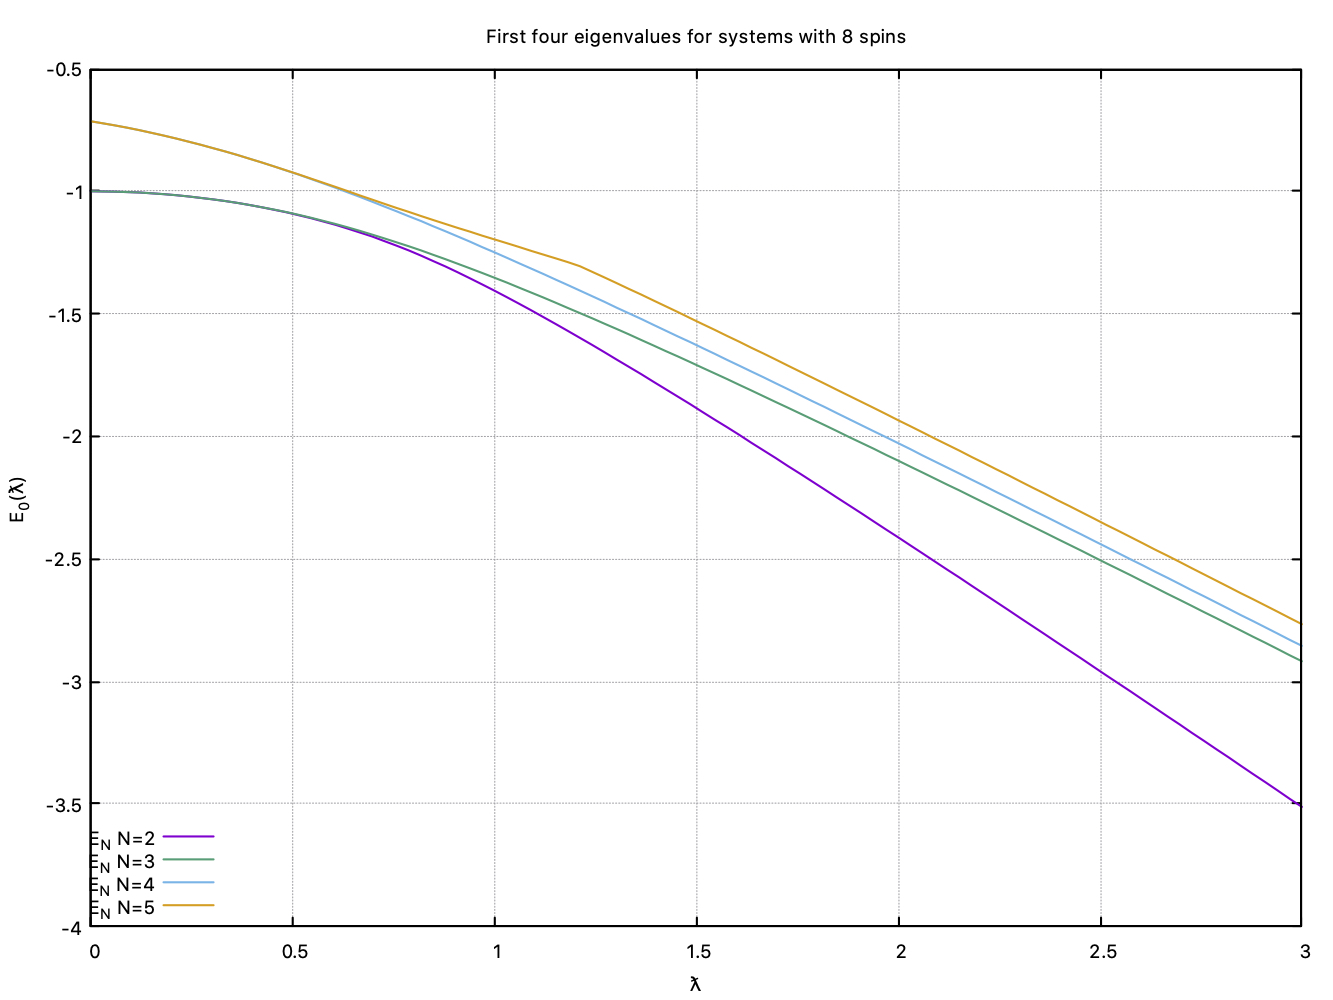
\includegraphics[width=.40\textwidth]{firstfour_8}\hfill
    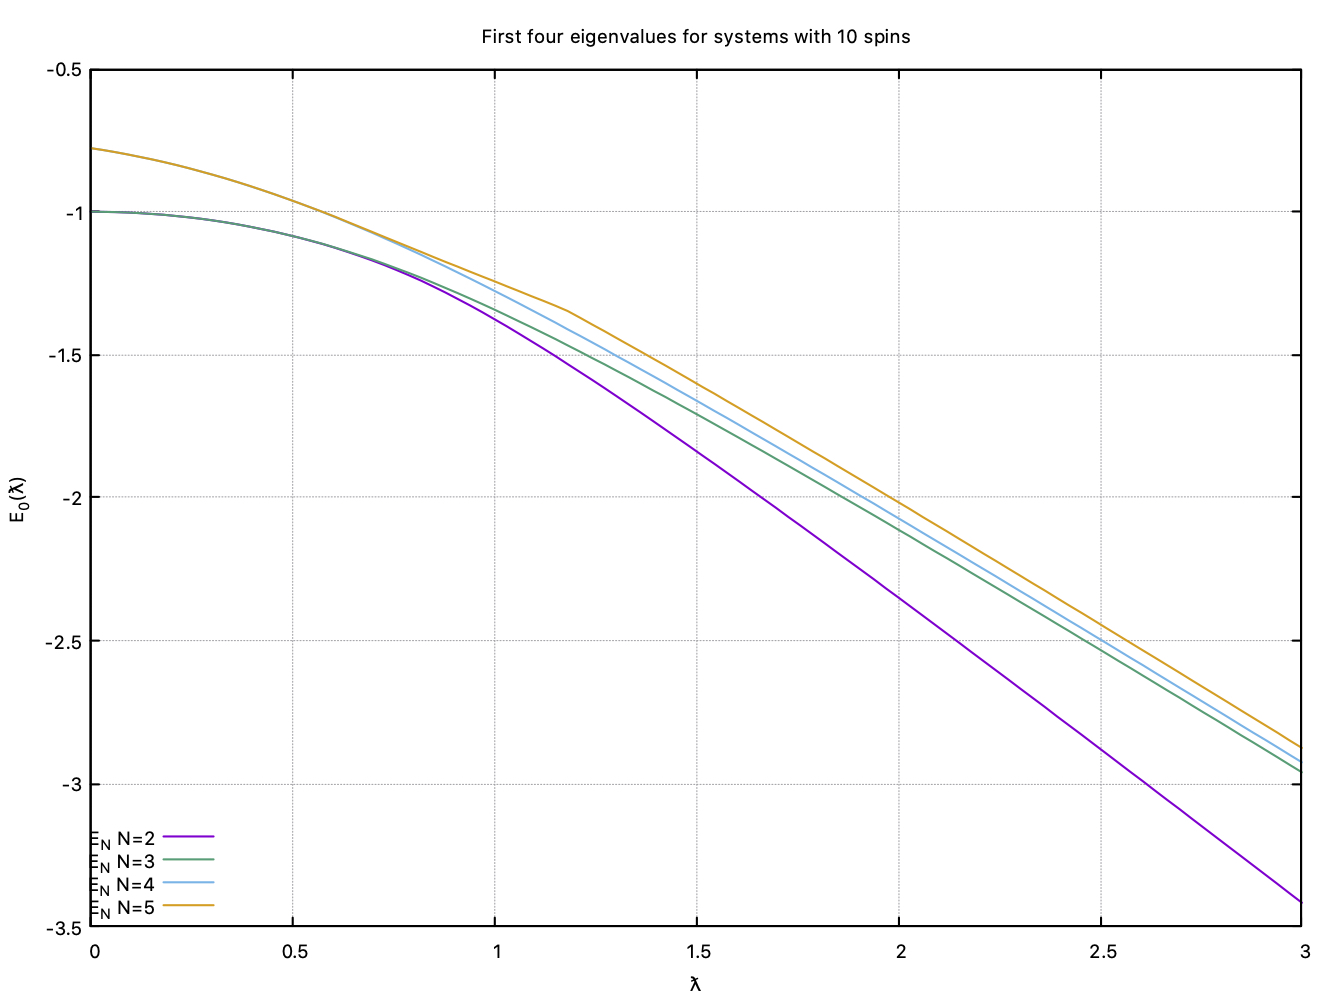
\includegraphics[width=.40\textwidth]{firstfour_10}\hfill
%%    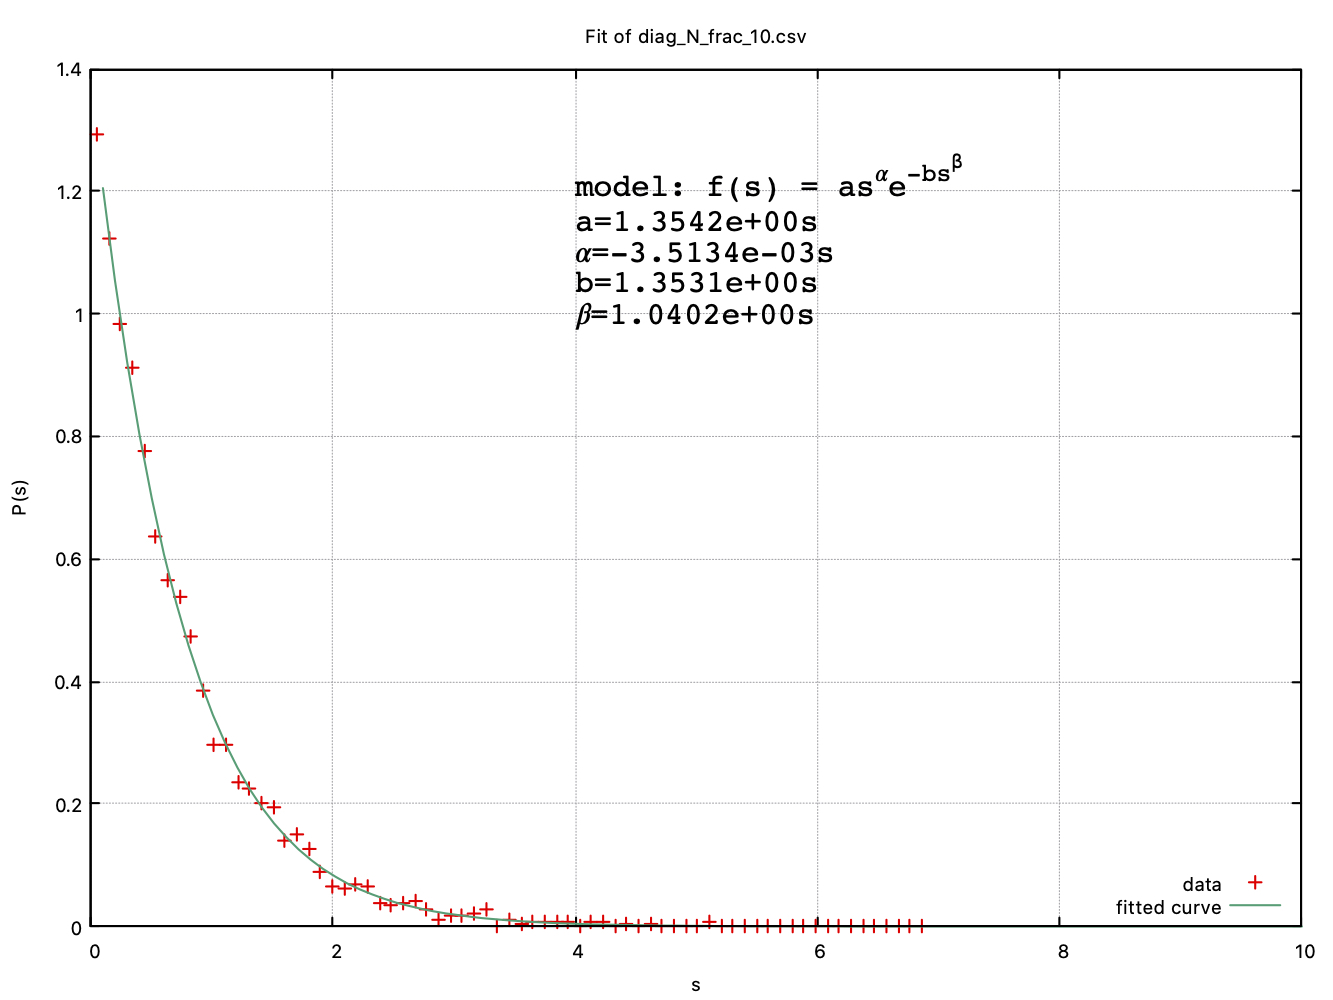
\includegraphics[width=.33\textwidth]{diag_N_frac_10}
    \caption{the first 4 eigenvalues of the system for different values of $N$ as a function of $\lambda$}\label{fig:foobar}
\end{figure}

\section{Self-evaluation}
I think the main objectives of the exercise are reached. I have learnt how to initialize and diagonalize the Ising hamiltonian.



\end{document}
